\documentclass{article}
\usepackage{graphicx, mathtools, amsmath, amssymb, dirtytalk, mathrsfs}
\graphicspath{{Images/}}

\setlength{\oddsidemargin}{0in}
\setlength{\textwidth}{6.5in}
\setlength{\topmargin}{-.55in}
\setlength{\textheight}{9in}
\pagestyle{empty}


\title{Optimization Midterm 2}
\author{Michael Nameika}
\date{April 2023}

\begin{document}

\maketitle

\begin{itemize}
    \item[1.] \textbf{Guaranteeing Convergence}
    \newline\newline
    Consider the function
    \[f(x) = 2(x_1 - 1)^2 + 10(x_2 - 2)^2,\]
    whose minimum clearly occurs at $(x_1, x_2) = (1,2)$. 
    \newline
    The following questions related to choosing a line search update, $x_1$. Consider the initial guess $x_0 = (0,0)^T$. All questions below use the search direction $p = (1,1)^T$ and some step length $\alpha > 0$. 
    \begin{itemize}
        \item[(a)] Show that this is a descent direction.
        \newline\newline
        To begin, let us find the gradient of $f$:
        \[\nabla f(x) = \begin{pmatrix}
            4(x_1 - 1)\\
            20(x_2 - 2)
        \end{pmatrix}\]
        and so at $x_0 = (0,0)^T$, $\nabla f(x_0) = (-4, -20)$. For $p$ to be a direction of descent, we require $p^T\nabla f(x_0) < 0$. Notice
        \begin{align*}
            p^T\nabla f(x_0) &= (1,1)\begin{pmatrix*}[r]
                -4\\
                -40
            \end{pmatrix*}\\
            &= -44 < 0.
        \end{align*}
        So $p$ is a descent direction.
        
        \item[(b)] For which value of $\epsilon$ does this direction satisfy the sufficient descent criteria?
        \newline\newline
        Recall that a search direction must satisfy the sufficient descent condition given by
        \[-\frac{p^T\nabla f(x_0)}{\|p\| \cdot \|\nabla f(x_0)\|} \geq \epsilon > 0\]
        Here, we have $p^T\nabla f(x_0) = -44$ and $\|p\| = \sqrt{2}$, $\|\nabla f(x_0)\| = 4\sqrt{101}$, so we require
        \[0 < \epsilon \leq \frac{11}{\sqrt{202}}\]

        \item[(c)] For which value of $m$ does this direction satisfy the gradient related criteria?
        \newline\newline
        Recall that for the gradient related condition, we require
        \[\|p\| \geq m\|\nabla f(x_0)\| \hspace{0.7em} \textit{for all k (with $m > 0$)}\]
        Here, $\|p\| = \sqrt{2}$ and $\|\nabla f(x_0) \| = 4\sqrt{101}$, so we require
        \begin{align*}
            \sqrt{2} &\geq m(4\sqrt{101})\\
            m &\leq \frac{\sqrt{2}}{4\sqrt{101}}\\
            m &\leq \frac{1}{2\sqrt{202}}
        \end{align*}
        That is, we require
        \[0 < m \leq \frac{1}{2\sqrt{202}}\]

        \item[(d)] For what range of $\alpha$ values does this update satisfy the Armijo condition when $\mu = 2/44$?
        \newline\newline
        Recall that the Armijo condition requires that $\alpha > 0$ must satisfy
        \[f(x_0 + \alpha p) \leq f(x_0) + \mu \alpha p^T\nabla f(x_0)\]
        Here, $f(x_0) = 42$, $p^T\nabla f(x_0) = -44$, and $f(x_0 + \alpha p) = f(\alpha p) = 12\alpha^2 - 44\alpha + 42$. That is, we require
        \begin{align*}
            12\alpha^2 - 44\alpha + 42 &\leq 42 - 2\alpha\\
            12\alpha^2 - 42\alpha &\leq 0\\
            \alpha(2\alpha - 7) \leq 0\\
            \alpha \leq \frac{7}{2}
        \end{align*}
        That is, to satisfy the Armijo conditions when $\mu = 2/44$, we require
        \[0 < \alpha \leq \frac{7}{2}\]
        

        \item[(e)] For what range of $\alpha$ values does this update satisfy the Wolfe condition when $\eta = 40/44$?
        \newline\newline
        Recall the Wolfe condition:
        \[|p^T\nabla f(x_0 + \alpha p)| \leq \eta |p^T\nabla f(x_0)|\]
        For $\eta = 40/44$, we have $\eta |p^T \nabla f(x_0)| = 40$ and notice that $|p^T\nabla f(x_0 + \alpha p)| = |24\alpha - 44|$. That is, we require
        \begin{align*}
            &|24\alpha - 44| \leq 40\\
            -40 &\leq 24\alpha - 44 \leq 40\\
            4 &\leq 24\alpha \leq 84\\
            \frac{1}{6} &\leq \alpha \leq \frac{7}{2}
        \end{align*}
        That is, when $\eta = 40/44$, to satisfy the Wolfe condition, we require
        \[\frac{1}{6}\leq \alpha \leq \frac{7}{2}\]
    \end{itemize}
    \pagebreak
    \item[2.] \textbf{Steepest-descent}
    \newline\newline
    Consider the problem
    \[\text{minimize} \hspace{1em} f(x) = \frac{1}{2}x^TQx - c^Tx,\]
    where $Q$ is a positive-definite matrix. Let $x_*$ be the minimizer of this function. Let $v$ be an eigenvecctor of $Q$, and let $\lambda$ be the associated eigenvalue. Suppose now that the starting point for the steepest-descent algorithm is $x_0 = x_* + v$.
    \begin{itemize}
        \item[(a)] Show that the gradient at $x_0$ is $\nabla f(x_0) = \lambda v$.
        \newline\newline
        Notice that the gradient of $f$ is given as
        \[\nabla f(x) = Qx - c\]
        Since $x_*$ is assumed to be the minimizer of $f$, we have $\nabla f(x_*) = 0$. Then plugging in $x_0$, we find
        \begin{align*}
            \nabla f(x_0) &= Qx_0 - c\\
            &= Q(x_* + v) - c\\
            &= Qx_* - c + Qv\\
            &= \lambda v
        \end{align*}
        which is what we wanted to show.
        \newline

        \item[(b)] Prove that if the steepest-descent direction is taken, then the step length which minimizes $f$ in this direction is $\alpha_0 = 1/\lambda$.
        \newline\newline
        \textbf{Proof}: Recall that the steepest-descent direction is given by the negative gradient. That is, for a search direction $p$, $p = -\nabla f(x)$ is the direction of steepest descent. We wish to find the step length that minimizes $f$ in this direction. That is, we wish to solve
        \begin{align*}
            \underset{\alpha > 0}{\text{minimize}} \hspace{1em} &f(x+\alpha p)
        \end{align*}
        Let $F(\alpha) = f(x + \alpha p)$. Then we wish to find $\alpha$ such that $F'(\alpha) = 0$. Notice
        \[F'(\alpha) = p^T\nabla f(x + \alpha p) = 0\]
        and that
        \begin{align*}
            p^T\nabla f(x_0 + \alpha p) &= p^T(Q(x_0 + \alpha p) - c)\\
            &= p^TQx_0 - c + \alpha p^TQp\\
            &= p^T\nabla f(x_0) + \alpha p^TQp\\
            &= \lambda p^Tv + \alpha p^TQp\\
            &= 0.
        \end{align*}
        Using $p = -\nabla f(x_0) = -\lambda v$, we find
        \begin{align*}
            \alpha (-\lambda v)^TQ(-\lambda v) &= \lambda^2 \|v\|^2\\
            \alpha &= \frac{\lambda^2\|v\|^2}{\lambda^2v^TQv}\\
            &= \frac{\lambda^2\|v\|^2}{\lambda^2v^T(\lambda v)}\\
            &= \frac{\lambda^2\|v\|^2}{\lambda^3\|v\|^2}\\
            &= \frac{1}{\lambda}.
        \end{align*}
        So $\alpha = 1/\lambda$, which is what we sought to show.
        \newline
        
        \item[(c)] Prove that the steepest-descent direction with an accurate step length will lead to the minimum of the function $f$ in one iteration.
        \newline\newline
        \textbf{Proof}: Using the initial guess of $x_0$, and steepest descent with step size $1/\lambda$ as given in part (a) and (b), we find
        \begin{align*}
            f(x_0 + \alpha p) &= f(x_* + v - 1/\lambda(\lambda v))\\
            &= f(x_* + v - v)\\
            &= f(x_*)
        \end{align*}
        So we find the minimum of $f$ in one iteration. 
        \newline
        
        \item[(d)] Confirm this result for the function
        \[f(x) = 3x_1^2 - 2x_1x_2 + 3x_2^2 + 2x_1 - 6x_2.\]
        Suppose the starting point is $x_0 = (1,2)^T$; compute the point obtained by one iteration of the steepest-descent algorithm. Prove that the point obtained is the unique minimum $x_*$. Verify that $x_0 - x_*$ is an eigenvector of the Hessian matrix.
        \newline\newline
        Rewriting the function as a quadratic form $f(x) = \tfrac{1}{2}x^TQx - c^Tx$, we find
        \[f(x) = \frac{1}{2}(x_1,x_2)\begin{pmatrix*}[r]
            6 & -2\\
            -2 & 6
        \end{pmatrix*}\begin{pmatrix}
            x_1\\
            x_2
        \end{pmatrix} - (-2,6)\begin{pmatrix}
            x_1\\
            x_2
        \end{pmatrix}\]
        with gradient
        \[\nabla f(x) = Qx - c\]
        It can be easily shown that the eigenvalues of $Q$ are $\lambda_1 = 4$ and $\lambda_2 = 8$. Use $\alpha = 1/\lambda_1$. The next value $x_1$ in the steepest descent algorithm will be given by
        \[x_1 = x_0 - \frac{1}{4}\nabla f(x_0)\]
        Notice that $\nabla f(x_0) = (4,4)^T$ and we find
        \begin{align*}
            x_1 &= \begin{pmatrix}
                1\\
                2
            \end{pmatrix} - 
            \frac{1}{4} \begin{pmatrix}
                4\\
                4
            \end{pmatrix}\\
            &= \begin{pmatrix}
                0\\
                1
            \end{pmatrix}
        \end{align*}
        And notice that 
        \[\nabla f(0,1) = \begin{pmatrix}
            0\\
            0
        \end{pmatrix}\]
        So $x_1 = (1,1)^T$ is the minimizer of $f$. To verify $x_0 - x_1 = (1,1)^T$ is an eigenvector of the Hessian $Q$, notice
        \begin{align*}
            \begin{pmatrix*}[r]
                6 & -2\\
                -2 & 6
            \end{pmatrix*}\begin{pmatrix}
                1\\
                1
            \end{pmatrix} &= 
            \begin{pmatrix}
                4\\
                4
            \end{pmatrix}\\
            &= 4\begin{pmatrix}
                1\\
                1
            \end{pmatrix}\\
            &= \lambda_1 (x_0 - x_1)
        \end{align*}    
    \end{itemize}
    

    \item[3.] \textbf{Linear Equality Constraints}
    \newline\newline
    Consider the problem of finding the minimum distance from a point $r$ to a set $\{x : a^Tx = b\}.$ Take $a^T$ to be a row vector. The problem can be expressed as
    \begin{align*}
        \text{minimize} \hspace{1em} &f(x) = \frac{1}{2}(x - r)^T(x - r)\\
        \text{subject to} \hspace{1em} &a^Tx = b.
    \end{align*}
    \begin{itemize}
        \item[(a)] Prove that the solution is given by
        \[x_* = r + \frac{b - a^Tr}{a^Ta}a.\]
        \textbf{Proof}: For a stationary point $x_*$ of $f$ over the given constraint, we require
        \[\nabla f(x_*) = a\lambda_*\]
        where $\lambda_* \geq 0$ is a Lagrange multiplier. Notice that $\nabla f(x_*) = x_* - r$. That is,
        \begin{align*}
            x_* - r &= \lambda_*a\\
            x_* &= \lambda_*a + r
        \end{align*}
        Additionally, from the constraint, we have $a^Tx = b$, so using the fact that $x_* - r = \lambda_*a$, we find
        \begin{align*}
            a^Tx_* &= \lambda_*a^Ta + a^Tr\\
            &= b\\
            \lambda_*a^Ta &= b - a^Tr\\
            \lambda_* &= \frac{b - a^Tr}{a^Ta}
        \end{align*}
        And so we find that the minimizer is given by
        \[x_* = r + \frac{b - a^Tr}{a^Ta}a\]
        Which is what we sought to show.

        \item[(b)] Prove that this point is a strict minimizer.
        \newline\newline
        Notice that $\nabla^2f(x) = I$, which is positive definite, so the second order sufficient condition is automatically satisfied, meaning that this point is a strict minimizer.
        \newline

        \item[(c)] Use part (a) to find where on the line $x_2 = 1 + x_1$ is closest to the point $r = (-1,1)^T$.
        \newline\newline
        Rewriting the equation of the line, we have
        \begin{align*}
            -x_1 + x_2 &= 1
        \end{align*}
        Which is our constraint $a^Tx = b$ with $a = (-1,1)^T$ and $b = 1$. Then using the formula we found in part (a), we have
        \begin{align*}
            x_* &= \begin{pmatrix*}[r]
                -1\\
                1
            \end{pmatrix*} + 
            \frac{1 - 2}{2}\begin{pmatrix*}[r]
                -1\\
                1
            \end{pmatrix*}\\
            &= \begin{pmatrix*}[r]
                -1/2\\
                1/2
            \end{pmatrix*}
        \end{align*}
        So the point on the line $x_2 = 1 + x_1$ that is closest to $(-1,1)^T$ is $x_* = (-1/2,1/2)$.
        \newline
        \item[(d)] Make a sketch.
        \newline\newline
        \begin{align*}
            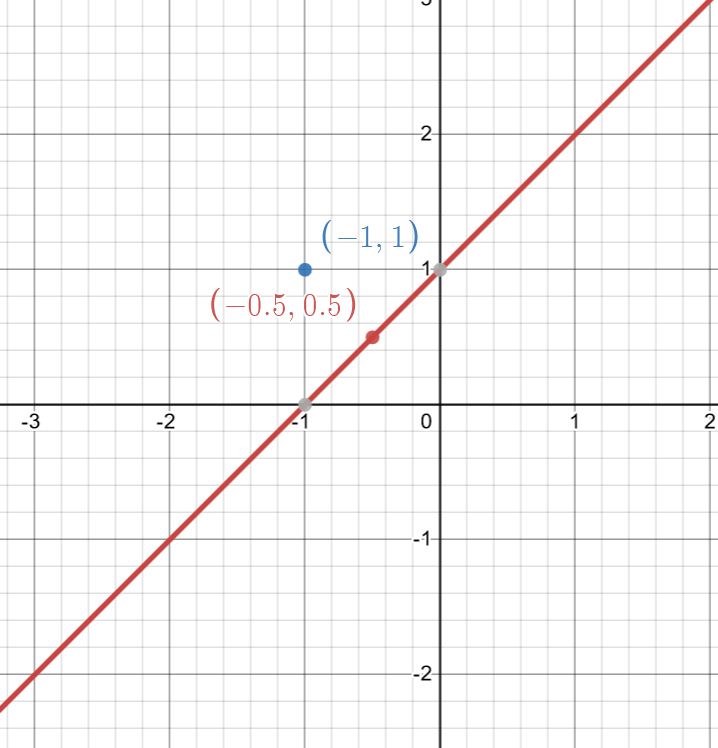
\includegraphics[scale = 0.7]{prob3sketch}
        \end{align*}
        
    \end{itemize}
\pagebreak
    \item[4.] \textbf{Nonlinear Inequality Constraints}
    \newline\newline
    Consider the problem
    \begin{align*}
        &f(x) = x_1^2 - x_2^2\\
        \text{subject to} \hspace{1em} &x_1^2 + x_2^2 \leq 1\\
        &x_1 + x_2 \geq 0
    \end{align*}
    \begin{itemize}
        \item[(a)] Make a sketch of the feasible region.
        \newline\newline
        \begin{center}
            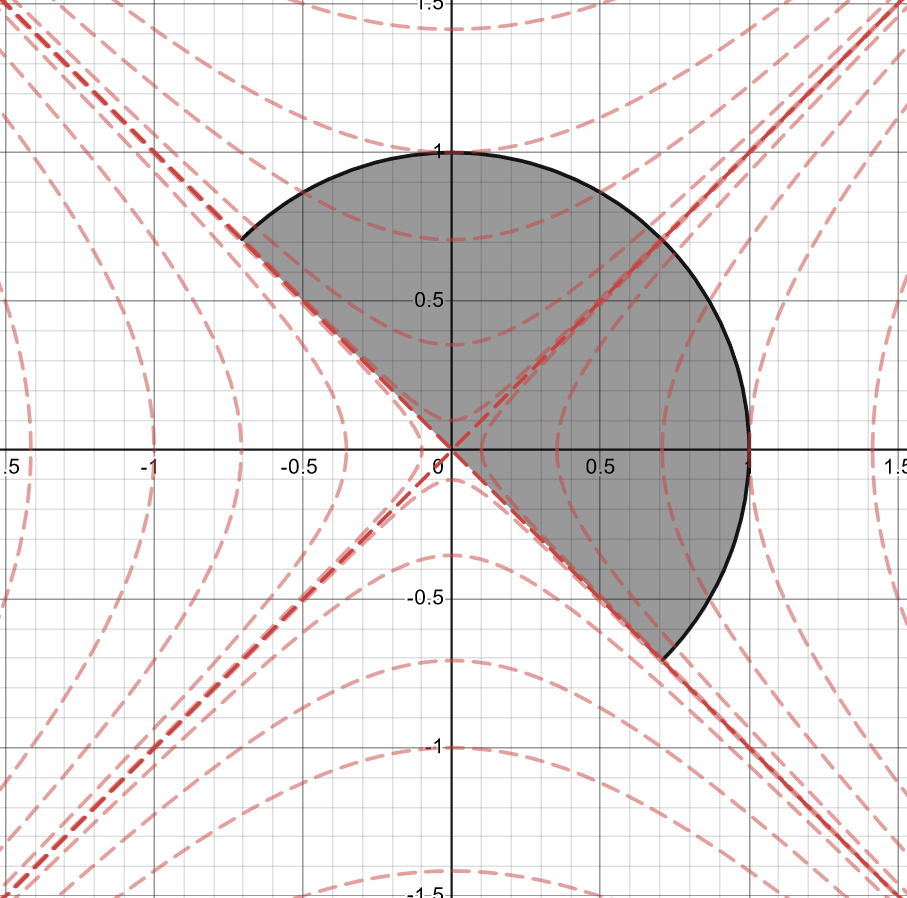
\includegraphics[scale = 0.6]{feasibleRegion4}
        \end{center}

        \item[(b)] Find all minimizers, maximizers, and saddle points.
        \newline\newline
        Begin by rewriting the constraints in the \say{$\geq 0$} form:
        \begin{align*}
            g_1(x) &= 1 - x_1^2 - x_2^2 \geq 0\\
            g_2(x) &= x_1 + x_2 \geq 0
        \end{align*}
        and define the Lagrangian 
        \begin{align*}
            \mathscr{L}(x,\lambda) &= f(x) - \lambda^Tg(x)\\
            &= x_1^2 - x_2^2 - \lambda_1(1 - x_1^2 - x_2^2) - \lambda_2(x_1 + x_2)
        \end{align*}
        At a stationary point, we require $\nabla_x\mathscr{L}(x,\lambda) = 0$. That is,
        \[\nabla_x\mathscr{L}(x,\lambda) = \begin{pmatrix}
            2x_1 + 2\lambda_1x_1 - \lambda_2\\
            -2x_2 + 2\lambda_1x_2 - \lambda_2
        \end{pmatrix} = \begin{pmatrix}
            0\\
            0
        \end{pmatrix}.\]
        We consider the following cases:
        \newline\newline
        \textbf{Case 1}: Both constraints are inactive. Then $\lambda_1 = \lambda_2 = 0$ and so $x_1 = x_2 = 0$, meaning the second constraint must be active, contradicting our assumption that both constraints were inactive.
        \newline\newline
        \textbf{Case 2}: Both constraints are active.
        \newline
        Then $x_1 + x_2 = 0$ and $x_1^2 + x_2^2 = 1$. From this, we get two possible values for $x$:
        \[x = \begin{pmatrix}
            \pm 1/\sqrt{2}\\
            \mp 1/\sqrt{2}
        \end{pmatrix}\]
        \begin{itemize}
            \item[(i)] Check $x = (-1/\sqrt{2}, 1/\sqrt{2})^T$:
            \newline
            From this, we find $\lambda_1 = 0$, $\lambda_2 = -\sqrt{2}$ meaning that this may be a local max. Now let us check the second order necessary conditions. At this point, the first constraint is degenerate, so we must find a null space matrix for the first row of the Jacobian of $g$ at this point. The Jacobian of $g$ is given by
            \[\nabla g(x) = \begin{pmatrix}
                -2x_1 & -2x_2\\
                1 & 1
            \end{pmatrix}\]
            so at the point $x = (-1/\sqrt{2}, 1/\sqrt{2})$, 
            \[\nabla g(-1/\sqrt{2}, 1/\sqrt{2}) = \begin{pmatrix}
                \sqrt{2} & -\sqrt{2}\\
                1 & 1
            \end{pmatrix}\]
            And a nullspace matrix for the first row is simply $Z = (1,1)^T$. Now, the Hessian of $\mathscr{L}(x,\lambda)$ is given by
            \[\nabla_{xx}^2\mathscr{L}(x,\lambda) = \begin{pmatrix}
                2 + 2\lambda_1 & 0\\
                0 & -2 + 2\lambda_1
            \end{pmatrix}\]
            And since $\lambda_1 = 0$, the Hessian of $\mathscr{L}(x,\lambda)$ is 
            \[\nabla_{xx}^2\mathscr{L}(x,\lambda) = \begin{pmatrix*}[r]
                2 & 0\\
                0 & -2
            \end{pmatrix*}\]
            Now checking $Z^T\nabla_{xx}^2\mathscr{L}(x,\lambda)Z$, we have
            \begin{align*}
                Z^T\nabla_{xx}^2\mathscr{L}(x,\lambda)Z &= (1,1)\begin{pmatrix*}[r]
                    2 & 0\\
                    0 & -2
                \end{pmatrix*}\begin{pmatrix}
                    1\\
                    1
                \end{pmatrix}\\
                &= (1,1)\begin{pmatrix*}[r]
                    2\\
                    -2
                \end{pmatrix*}\\
                &= 0
            \end{align*}
            So the sufficiency conditions are not satisfied. Let us instead think about making a small movement interior to the domain to determine if this is a local maximum. Consider moving a small amount $\delta_1 > 0$ in the $x_1$ direction and $\delta_2$ in the $x_2$ direction. To begin, let us consider the point $x = \left(-\frac{1}{\sqrt{2}} + \delta_1, \frac{1}{\sqrt{2}} + \delta_2\right)$. Factoring our objective function, we find
            \[f(x) = x_1^2 - x_2^2 = (x_1 - x_2)(x_1 + x_2)\]
            at our perturbed point, we have
            \begin{align*}
                f(x+\delta) &= (-\sqrt{2} + \delta_1 - \delta_2)(\delta_1 + \delta_2)
                < 0
            \end{align*}
            for values of $\delta_1,\delta_2$ such that $x + \delta$ remains in the feasible region. Similarly, we can show the same for a perturbation $\delta_2$ in the negative $x_2$ direction. That is, $x = (-\tfrac{1}{\sqrt{2}},\tfrac{1}{\sqrt{2}})$ is a local maximum. 

            \item[(ii)] Check $x = (1/\sqrt{2},-1/\sqrt{2})^T$
            \newline
            Similar to part (i), we have $\lambda_2 = \sqrt{2}$ and $\lambda_1 = 0$. Notice now that 
            \[\nabla g(1/\sqrt{2},-1/\sqrt{2}) = \begin{pmatrix}
                \sqrt{2} & -\sqrt{2}\\
                1 & 1
            \end{pmatrix}\]
            So similar to part (i), $Z = (1,1)^T$. Notice that the second order sufficiency condition $Z^T\nabla_{xx}^2\mathscr{L}(x,\lambda)Z$ is the same in this case, which is just zero, meaning that the sufficiency conditions are not satisfied. Similar as in part (i), we can show that the point $x = (\tfrac{1}{\sqrt{2}},-\tfrac{1}{\sqrt{2}})$ is a local minimum.
            \newline
        \end{itemize}
        
        \textbf{Case 3}: The first constraint is active. 
        \newline
        Then $\lambda_2 = 0$ and $x_1^2 + x_2^2 = 1$. 
        \newline
        From the gradient of $\mathscr{L}$, we have 
        \begin{align*}
            x_2 &= \lambda_1 x_2\\
            -x_1 &= \lambda_1 x_1
        \end{align*}
        Using this in combination with the first constraint being active, we find 
        \[\lambda_1 = \pm 1\]
        \begin{itemize}
            \item[i)] Suppose $\lambda_1 = -1$. Then $x_2 = 0$ and $x_1 = \pm 1$. The point $x = (-1,0)^T$ is infeasible, so $x_1 = 1$. 
            \newline
            At this point,
            \begin{align*}
                \nabla g(1,0) &= \begin{pmatrix*}[r]
                    -2 & 0\\
                    1 & 1
                \end{pmatrix*}\\
                \nabla_{xx}^2\mathscr{L}(x,\lambda) &= \begin{pmatrix*}[r]
                    0 & 0\\
                    0 & -4
                \end{pmatrix*}
            \end{align*}      
            Notice that $Z = (1,-1)^T$ is a null space matrix for the degenerate constraint (constraint 2), so checking the reduced Hessian, we find
            \begin{align*}
                Z^T\nabla_{xx}^2\mathscr{L}(x,\lambda)Z &= (1,-1)\begin{pmatrix*}[r]
                    0 & 0\\
                    0 & -4
                \end{pmatrix*}\begin{pmatrix*}[r]
                    1\\
                    -1
                \end{pmatrix*}\\
                &= (1,-1)\begin{pmatrix*}[r]
                    0\\
                    4
                \end{pmatrix*}\\
                &= -4 < 0
            \end{align*} 
            So $x = (1,0)^T$ is a strict local maximizer.

            \item[ii)] Check $\lambda_1 = 1$. Then $x_1 = 0$ and $x_2 = 1$ by similar reasoning as in part i). At this point, we have for $\nabla g(x)$ and $\nabla_{xx}^2\mathscr{L}(x,\lambda)$:
            \begin{align*}
                \nabla g(0,1) &= \begin{pmatrix*}[r]
                    0 & -2\\
                    1 & 1
                \end{pmatrix*}\\
                \nabla_{xx}^2\mathscr{L}(x,\lambda) &= \begin{pmatrix*}[r]
                    4 & 0\\
                    0 & 0
                \end{pmatrix*}
            \end{align*}
            And notice that $Z = (1,0)^T$ is a nullspace matrix for the degenerate constraint (constraint 1), so checking the reduced Hessian, we find
            \begin{align*}
                Z^T\nabla_{xx}^2\mathscr{L}(x,\lambda)Z &= (1,0)\begin{pmatrix*}[r]
                    4 & 0\\
                    0 & 0
                \end{pmatrix*}\begin{pmatrix}
                    1\\
                    0
                \end{pmatrix}\\
                (1,0)\begin{pmatrix}
                    4\\
                    0
                \end{pmatrix}\\
                &= 4 > 0
            \end{align*}
            So $x = (0,1)^T$ is a strict local minimizer.
        \end{itemize}
        \textbf{Case 4}: The second constraint is active. 
        \newline
        Then $\lambda_1 = 0$ and $x_1 + x_2 = 0$. 
        \newline
        From the reduced gradient, we find
        \begin{align*}
            \lambda_1 = 2x_1\\
            \lambda_1 = -2x_2
        \end{align*}
        which gives us the same information as the second constraint. That is, every point on the second constraint is a stationary point (?). A point of interest is the point $x = (0,0)^T$ since here, $\lambda_1 = 0$, and the first order sufficiency condition is satisfied. At this point, the gradient of the constraints and the reduced Hessian are as follows:
        \begin{align*}
            \nabla g(0) &= \begin{pmatrix}
                0 & 0\\
                1 & 1
            \end{pmatrix} \\
            \nabla_{xx}^2\mathscr{L}(0,\lambda) &= \begin{pmatrix*}[r]
                -2 & 0\\
                0 & 2
            \end{pmatrix*}
        \end{align*}
        Since both constraints are degenerate at this point, we must find a null space matrix for $\nabla g(0)$, which is simply $Z = (1,-1)^T$. Checking the second order sufficiency condition:
        \begin{align*}
            Z^T\nabla_{xx}^2\mathscr{L}(0,\lambda)Z &= (1,-1)\begin{pmatrix*}[r]
                -2 & 0\\
                0 & 2
            \end{pmatrix*}\begin{pmatrix*}[r]
                1\\
                -1
            \end{pmatrix*}\\
            &= 0
        \end{align*}
        So the second order conditions are not satisfied. Now, notice if a small perturbation is made in the positive $x_1$ direction, $f(\delta_1,0)  > f(0,0)$ and if a small perturbation is made in the positive $x_2$ direction, $f(0,\delta_2) < f(0,0)$, meaning that the point $(0,0)$ is a saddle point.
        \newline\newline
        Finally, we found that the point $x = (\frac{1}{\sqrt{2}}, -\frac{1}{\sqrt{2}})^T$ is a local minimum with an associated objective value of $f(x) = 0$. 
        Similarly, we found that the point $x = (-\frac{1}{\sqrt{2}}, \frac{1}{\sqrt{2}})^T$ is a local maximum with an associated objective value of $f(x) = 0$. 
        
        Next, the points $x = (0,1)^T$ and $x = (0,1)^T$ were strict local minimizers and maximizers, respectfully, with associated objective values of $f(x) = -1$, $f(x) = 1$.
        
        Finally, the point $x = (0,0)^T$ was shown to be a saddle point with an associate objective value of $f(x) = 0$.

        \item[(c)] Add the points from part (b) to your sketch.
        \newline\newline
        \begin{center}
            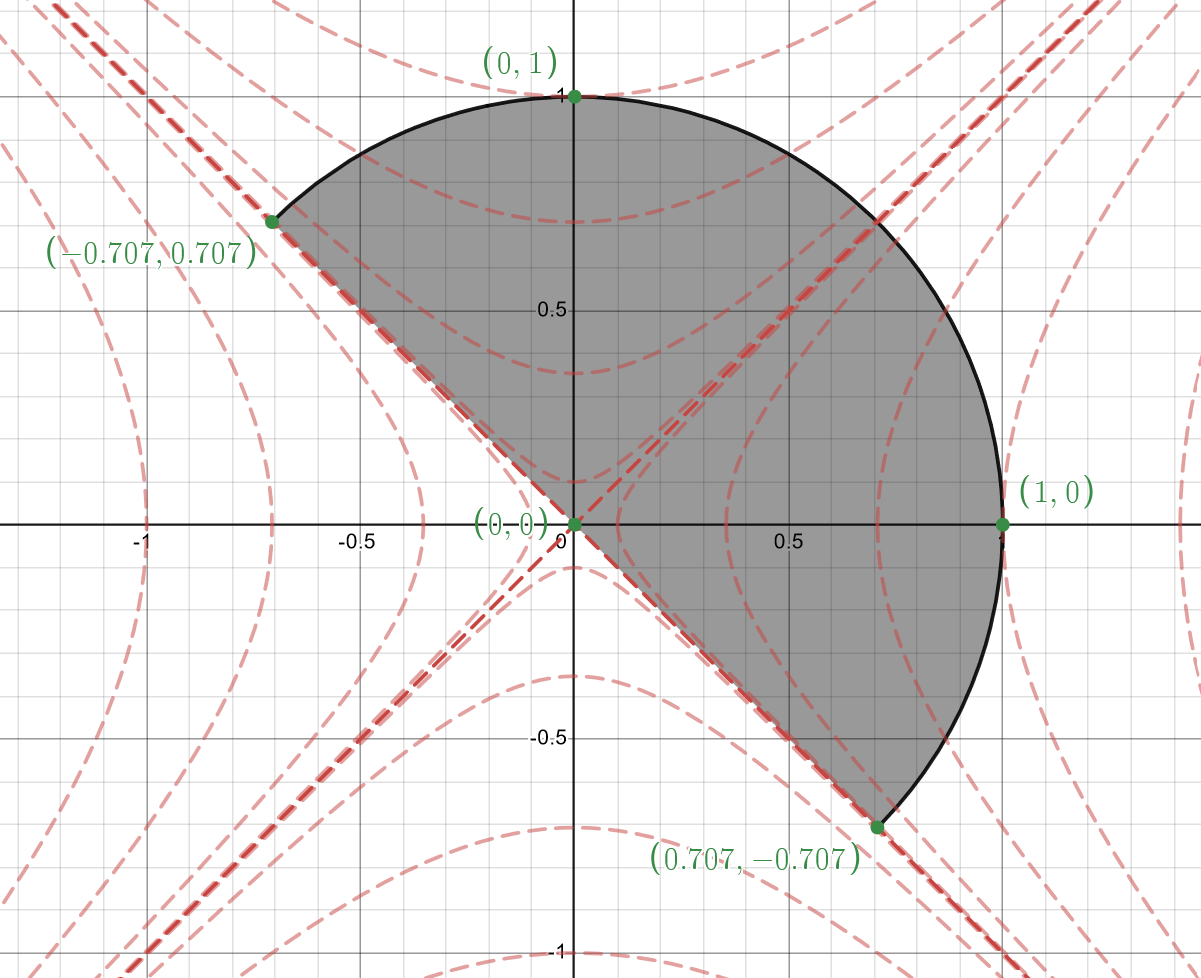
\includegraphics[scale = 0.5]{regionWithPoints}
        \end{center}
    \end{itemize}
    \pagebreak
    \item[5.] \textbf{Linear Objective, Quadratic Constraint}
    Consider the problem
    \begin{align*}
        \text{minimize} \hspace{1em} &f(x) = c^Tx\\
        \text{subject to} \hspace{1em} &x^TQx \leq 1,
    \end{align*}
    where $Q$ is a positive-definite symmetric matrix.
    \begin{itemize}
        \item[(a)] Solve the problem. Show that the optimality conditions are satisfied.
        \newline\newline
        Begin by rewriting the constraint to be of the \say{$\geq 0$} type. That is, our constraint is $1 - x^TQx \geq 0$. Building the Lagrangian, we have
        \[\mathscr{L} = f(x) - \lambda g(x)\]
        where $\lambda$ is the problem's Lagrange multiplier and $g(x) = 1 - x^TQx \geq 0$. For a stationary point to exist, we require $\nabla_x\mathscr{L} = 0$. That is,
        \begin{align*}
            \nabla_x\mathscr{L} &= c + \lambda Qx = 0\\
            \lambda Qx &= -c.
        \end{align*}
        Notice that if the constraint is inactive, $\lambda = 0$ and $\nabla_x \mathscr{L} = 0$ if and only if $c = 0$. If $c = 0$, the problem is not of interest since $f \equiv 0$. 
        Then we require that the constraint is active. Thus, for a minimizer, we find (using the fact that $Q$ is positive definite, so $Q^{-1}$ exists):
        \[x_* = -\frac{1}{\lambda}Q^{-1}c\]
        Further, since the constraint is active, we have $x_*^TQx_* = 1$. Using the above value for $x_*$, we find
        \begin{align*}
            \left(-\frac{1}{\lambda}Q^{-1}c\right)^TQ\left(-\frac{1}{\lambda}Q^{-1}c\right) &= 1\\
            \frac{1}{\lambda^2}c^TQ^{-1}QQ^{-1}c &=1\\
            \frac{1}{\lambda^2}c^TQ^{-1}c &= 1\\
            \lambda &= \pm \sqrt{c^TQ^{-1}c}
        \end{align*}
        At a minimum, we require $\lambda \geq 0$, so take $\lambda = \sqrt{c^TQ^{-1}c}$. 
        Additionally, since $Q$ is positive definite, $Q^{-1}$ is also positive definite, so $c^TQ^{-1}c > 0$ for all $c \neq 0$.
        Now, notice that $\nabla_{xx}^2\mathscr{L} = \lambda Q$ and since $\lambda > 0$, $\nabla_{xx}^2\mathscr{L}$ is positive definite, so the second order sufficiency condition is automatically satisfied. 
        (Alternatively, $\nabla g = Q$ which has only a trivial null space, so any basis for the null space is empty, also automatically satisfying the second order sufficiency condition.) Finally, our expression for $x_*$ is
        \[x_* = -\frac{Q^{-1}c}{\sqrt{c^TQ^{-1}c}}\]
        
        
        \item[(b)] What is the optimal objective value?
        \newline\newline
        Using the value for $x_*$ we found in part (a), we find
        \begin{align*}
            f(x_*) &= c^Tx_*\\
            &= -\frac{c^TQ^{-1}c}{\sqrt{c^TQ^{-1}c}}\\
            &= -\sqrt{c^TQ^{-1}c}
        \end{align*}

        \item[(c)] Use part (a) to find the minimizer of the function $f(x) = -x_1 + 3x_2$ subject to the constraint $2x_1^2 - 2x_1x_2 + 3x_2^2 \leq 1$.
        \newline\newline
        For this problem, we have
        \[c = (-1,3)^T, \hspace{1em} Q = \begin{pmatrix*}[r]
            2 & -1\\
            -1 & 3
        \end{pmatrix*}\]
        From our work in part (a) and (b), we find the minimizer
        \begin{align*}
            x_* &= -\frac{Q^{-1}c}{\sqrt{c^TQ^{-1}c}}\\
            &= \begin{pmatrix}
                0\\
                1/\sqrt{3}
            \end{pmatrix}
        \end{align*}
        with an associated function value of
        \begin{align*}
            f(x_*) &= -\sqrt{c^TQ^{-1}c}\\
            &= -\sqrt{3}
        \end{align*}
        
    \end{itemize}
\end{itemize}


\end{document}
